\section{Fey Corgi}

\begin{figure}
   \vspace*{-3.5cm}
   %\hspace*{-2cm}
   \makebox[\textwidth][c]{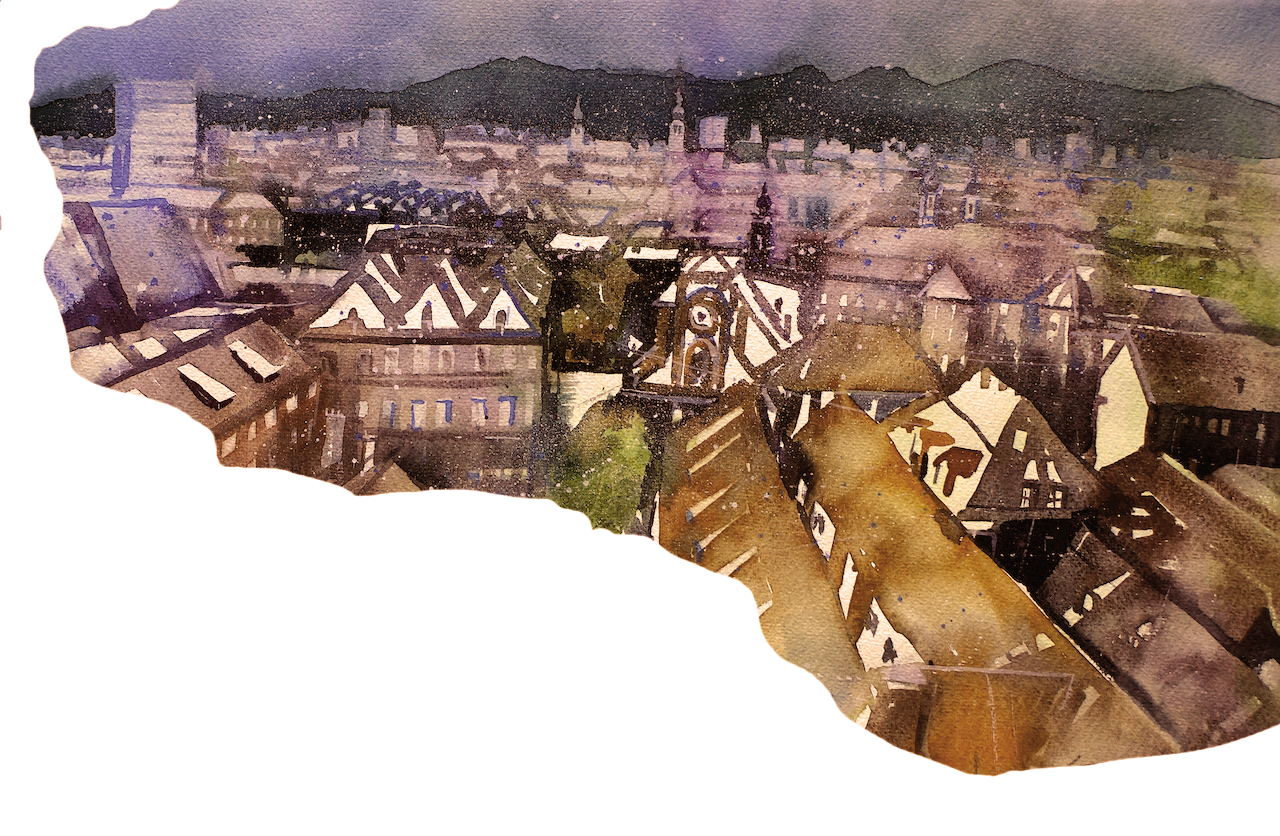
\includegraphics[width=1.1\pdfpagewidth]{2-Razze/2.2-FeyCorgi/Risorse/townbg.png}}
\end{figure}


\begin{figure}
  % \vspace*{-2cm}
   \hspace*{-10cm}
   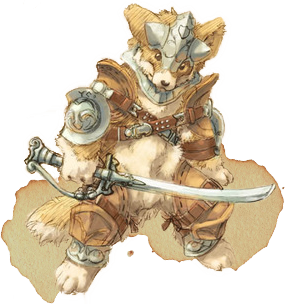
\includegraphics[width=10cm]{2-Razze/2.2-FeyCorgi/Risorse/fey_corgi2.png}
\end{figure}

\subsection{Viaggiatori dal Feywild}
I Fey Corgi sono, come intuibile dal nome, fate a tutti gli effetti. Molto rari a Midgard, vivono in piccole tribù nelle foreste del Feywild, assieme a spiriti della natura come driadi e ninfe.

La loro presenza a Midgard è lentamente cresciuta dopo lo Squarcio, ma i loro numeri sono ancora trascurabili, persino rispetto a tutte quelle creature maligne provenienti dallo stesso piano.

\subsection{Simili a Cani}
Pur dotati di un'intelligenza nettamente superiore, caratterialmente non sono dissimili dai Corgi del Primo Materiale: sono tendenzialmente amichevoli, amano stare tra la gente e si mescolano facilmente con altre culture e gruppi di altre razze intelligenti.

Sviluppano forti legami con coloro con cui passano molto tempo, anche con chi non li tratta con la dovuta gentilezza. Non è impossibile farli arrabbiare, ma è estremamente raro che finiscano per l'odiare qualcuno.

I Fey Corgi sono una specie molto curiosa, e arrivano anche a rubare e accumulare oggetti di poco valore, come calzini o biancheria: non è raro che la loro curiosità li faccia finire nei guai. Sono bassi, ma i loro sensi sviluppati li rendono ottimi avventurieri, in grado in caso anche di difendersi con i denti. Letteralmente.

\subsection{Nomi dei Fey-Corgi}
Per via della loro natura di fate i Fey Corgi sono estremamente gelosi dei loro veri nomi, per questo motivo, e per il naturale apprezzamento che hanno per i nomi dei cani delle razze di Midgard, che trovano esotici e gioiosi, tendono ad adottare semplici nomi canini:

\textit{\textbf{Nomi Maschili:}} Lucky, Rex, Spot, Rover, Buddy.

\textit{\textbf{Nomi Femminili:}} Sasha, Lucy, Bella, Lady.

\subsection{Tratti Raziali dei Fey Corgi}

In quanto Fey Corgi il tuo personaggio ha diverse capacità magiche e fisiche, dovute sia al suo retaggio fatato che canino.

\textit{\textbf{Aumento Abilità}} La tua Saggezza aumenta di 2.

\textit{\textbf{Età}} I Fey Corgi vivono un po' più dei cani comuni, e maturano un po' più lentamente. I Fey Corgi raggiungono tipicamente la maturità attorno ai due anni e tipicamente sopravvivono da 28 a 34 anni.

\textit{\textbf{Allineamento}} I Fey Corgi sono fortemente influenzati dall'ambiente sociale in cui crescono, ciononostante tendono generalmente più verso allineamenti buoni.

\textit{\textbf{Stazza}} I Fey corgi sono poco più grandi di quelli del piano materiale, aggirandosi attorno ai 3 o 4 piedi, solitamente tendenti al basso di queste misure. La tua taglia è piccola (small).

\textit{\textbf{Velocità}} I Fey Corgi sono in grado di muoversi facilmente sia a due che a quattro zampe, raggiungendo nel primo caso una velocità base di 25 piedi, e nel secondo di 35 piedi. Un Fey corgi che si muove a quattro zampe non potrà usare le zampe anteriori nel suo turno, potrà quindi attaccare solo con il morso.

\textit{\textbf{Scurovisione}} Essendo in parte cane hai una capacità superiore di vedere al buio. Vedi nella penombra come se fosse luce piena e nell'oscurità come fosse penombra entro 60 piedi. Non vedi i colori a qualunque luminosità, solo gradienti di grigio.

\textit{\textbf{Olfatto e Udito fini}} Avendo un olfatto e udito più acuti del normale sei proficente nella skill Percezione e hai vantaggio in tutti quei tiri che coinvolgono l'annusare o ascoltare.

\textit{\textbf{Natura Fatata}} Hai vantaggio sui tiri salvezza contro l'essere affascinato (charm) e non puoi essere addormentato magicamente

\textit{\textbf{Ladro-Batuffolo}} Come azione puoi compiere un attacco corpo a corpo. Se colpisci il bersaglio deve compiere un tiro salvezza sulla Forza con DC15 o essere buttato a terra (knocked prone) privo di un calzino. Questo aspetto non si applica se il bersaglio non indossa calzini. Ogni altro genere di calzatura non viene rimosso né offre protezione al calzino.

\textit{\textbf{Morso}} Puoi decidere di usare al più un attacco per turno per mordere un avversario. Esegui un attacco corpo a corpo, se colpisci infliggi 1d4+STR danni perforanti (piercing). Se vuoi puoi usare una bonus action per forzare una presa (grapple) sul tuo bersaglio. Se esegui la presa con successo l'avversario è buttato a terra (knocked prone)

\textit{\textbf{Lingue}} Sai parlare, leggere e scrivere il comune e la lingua della tua comunità. Se quella lingua è il comune, scegline pure un'altra. Puoi comunicare con i cani, tuttavia essi non hanno un vero linguaggio, e le informazioni che possono trasmettere sono minime.

\textit{\textbf{Sottorazze}} Più che in effettive sottorazze i Fey Corgi si suddividono in base alle rispettive comunità di appartenenza, che ne determinano la crescita: i Fey Corgi dei Boschi e i Fey Corgi Urbani.

\subsubsection{Fey Corgi dei Boschi}
Alcuni Fey Corgi si aggregano in piccole comunità in foreste che ricordano loro quelle del Feywild da cui provengono. Queste comunità tendono indirettamente ad attirare altra magia del Feywild, permettendo la crescita di funghi e fiori di quel piano, e attirando a volte anche Driadi e Ninfe, che apprezzano particolarmente la compagnia di questa specie.

\textit{\textbf{Aumento Abilità}} La tua destrezza aumenta di due punti.

\textit{\textbf{Maschera delle Selve}} Puoi tentare di nasconderti anche quando sei coperto leggermente da fogliame, pioggia intensa neve fitta, nebbia o altri fenomeni naturali.(Mask of the Wild)

\textit{\textbf{Addestramento nei Boschi}} Sei proficente con l'uso di Balestra leggera, balestra da braccio, arco corto, arco lungo e spada corta (hand crossbows, Longbows, Light Crossbows, Shortbows and Shortsword)

\textit{\textbf{Competenze naturali}} Sei proficente nella skill Natura (Nature).

\subsubsection{Fey Corgi Urbano}
I Fey Corgi Urbani apprezzano comunque i Boschi e la natura, ma, affascinati dalle grandi città e dalla frenesia delle razze del Primo Materiale si sono mescolati maggiormente con le culture del posto. La loro naturale curiosità li spinge a interessarsi di storia, tecnologia e tecniche rare nel Feywild.

\textit{\textbf{Aumento Abilità}} Il tuo punteggio di Intelligenza aumenta di 2.

\textit{\textbf{Interesse nell'artigianato}} Sei proficente in un attrezzo da artigiano (artisan tool) a tua scelta.

\textit{\textbf{Adorabile}} Sei competente nella Skill Persuasione (persuasion).

\textit{\textbf{Astuzia}} Sei competente nella Skill Ingannare (deception).

\begin{figure}[t]
  % \vspace*{-2cm}
  % \hspace*{-10cm}
   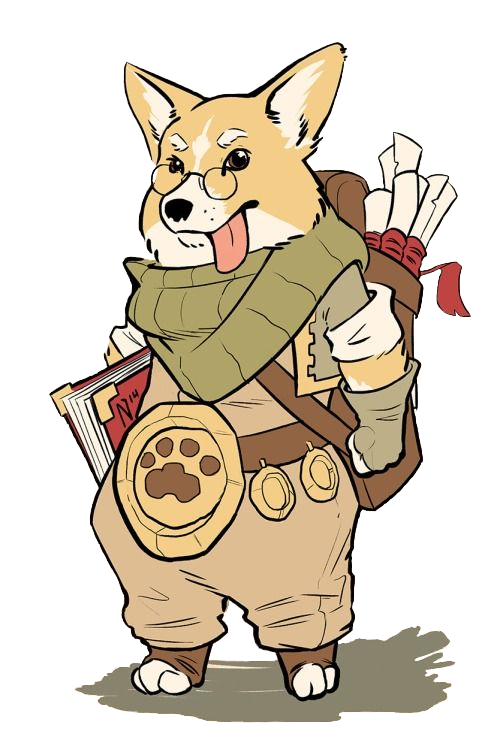
\includegraphics[height=10cm]{2-Razze/2.2-FeyCorgi/Risorse/Fey_Corgi3.png}
\end{figure}

\clearpage
